\chapter{Tecnologie utilizzate}\label{chp:02-technologies}
In questo capitolo sono descritte le tecnologie utilizzate per la realizzazione del progetto unitamente alle motivazioni legate all'uso 
di certi sistemi rispetto ad altri. In particolare viene fornita una panoramica dei sistemi di raccomandazione analizzati e studiati,
nel capitolo successivo vengono approfonditi a livello pratico i sistemi di raccomandazione Memory-based i quali sono stati utilizzati 
per l'implementazione della soluzione.
%
\section{Perché Python e Django}
\paragraph{Python}
Python è un linguaggio di programmazione ad alto livello, orientato agli oggetti, adatto, tra gli altri usi, a sviluppare applicazioni 
distribuite, scripting, computazione numerica e system testing; ideato e rilasciato pubblicamente per la prima volta nel 1991 dal suo 
creatore Guido van Rossum, programmatore olandese.\hfill\break
Python supporta diversi paradigmi di programmazione, come quello object-oriented (con supporto all'ereditarietà multipla), quello 
imperativo e quello funzionale, e offre una tipizzazione dinamica forte. È fornito di una standard library estremamente ricca, che, 
unitamente alla gestione automatica della memoria e a robusti costrutti per il controllo delle eccezioni, rendono Python uno dei linguaggi 
più ricchi e comodi da usare; inoltre è anche semplice da usare e imparare. 
Python, nelle intenzioni di Guido van Rossum, è nato per essere un linguaggio immediatamente intuibile. La sua sintassi è pulita e snella 
così come i suoi costrutti, decisamente chiari e non ambigui.\hfill\break
Un aspetto inusuale e unico di Python è il metodo che viene usato per delimitare i blocchi di codice.
%
\lstset{style=python_code_style}
\begin{lstlisting}[language=Python, caption={Esempio di programma scritto in Python}]
# Testing if two strings are equals
def test(got, expected):
    if got == expected:
        result = ' OK '
    else:
        result = ' X '
    print('%s got: %s expected: %s' % (result, repr(got), repr(expected)))

def main():
    test('hail', 'hailing')
    test('swiming', 'swimingly')
    test('do', 'do')

if __name__ == '__main__':
    main()
\end{lstlisting}
%
Nei linguaggi come Pascal, C e Perl, i blocchi di codice sono indicati con le parentesi oppure con parole chiave 
(il C e il Perl usano \textbf{{ }}; il Pascal usa \textbf{begin} ed \textbf{end}). In questi linguaggi è solo una convenzione degli sviluppatori il fatto di 
indentare il codice interno ad un blocco, per metterlo in evidenza rispetto al codice circostante. In Python invece di usare parentesi 
o parole chiave, si usa l'indentazione stessa per indicare i blocchi nidificati in congiunzione col carattere "due punti" (:). Si usa 
sia una tabulazione sia un numero arbitrario di spazi, ma lo standard Python è di 4 spazi.
Python è un linguaggio pseudocompilato: un interprete si occupa di analizzare il codice sorgente (semplici file testuali con 
estensione .py) e, se sintatticamente corretto, di eseguirlo, non esiste una fase di compilazione separata (come, per esempio, 
avviene in C, ) che generi un file eseguibile partendo dal sorgente \cite{python-documentation}.
%
\paragraph{Django}
Django è un web framework di alto livello basato su Pyhton che permette di sviluppare rapitamente e con tutti i presupposti per un sistema sicuro, un sito web
perfettamente mantenibile. Esso si occupa della maggiori difficoltà dello sviluppo web, così da permettere di concentrarsi sulla scrittura dell'app; inoltre 
è open-source e ha una comunità attiva, una documentazione completa e semplice da consultare.\hfill\break
Django aiuta a scrivere applicazioni con le seguenti caratteristiche \cite{django-documentation}.
\begin{description}
    \item[Versatile:] può essere usato per la creazione di quasi tutti i tipi di siti web, a partire da sistemi per la gestione di contenuti,
    a social network e siti di notizie; può lavorare con qualunque client-side framework, e gestire contenuti in quasi tutti i formati (inclusi HTML, 
    RSS feeds, JSON, Xml, etc). Internamente permette la scelta e l'implementazione di qualsiasi funzionalità (es. molti dei database più popolari, ecc.).
    \item[Sicuro:] aiuta gli sviluppatori a evitare gli errori più comuni in merito alla sicurezza provvedendo un framework costruito per eseguire 
    le operazioni in modo corretto e sicuro. Ad esempio, Django fornisce un metodo sicuro per gestire gli account degli utenti e le relative 
    password, evitando errori comuni come inserire informazioni riguardanti la sessione dell'utente nei cookies, dove sarebbero vulnerabili (invece i cookie 
    contengono soltanto una chiave, e i valori effettivi sono salvati nel database) o salvare direttamente una password invece di una hash password.
    \item[Mantenibile:] il codice di Django è scritto seguendo i principi e i pattern che incoraggiano la creazione di codice mantenibile e riusabile. Inoltre 
    particolare, fa uso del principio "Don't Repeat Yourself" (DRY) così da ridurre al minimo le duplicazioni non necessarie, diminuendo la quantità di codice.
    Django raggruppa parti di codice letto in moduli seguendo le linee guida del pattern Model View Controller (MVC).
    \item[Portabile:] Django essendo scritto in Python, un linguaggio multi piattaforma, lo rende indipendente dal sistema operativo eseguito sul server, che 
    sia Linux, Windows o Mac OS X. Per di più, Django è ben supportato da molti web hosting provider, che spesso provvedono a specifche infrastrutture
    e documentazione per l'hosting di siti web in Django.
\end{description}
In generale, un tradizionale server web resta in attesa di richieste HTTP da parte del browser web (o altri client) degli utenti; nel momento in cui riceve 
una richiesta (solitamente di tipo POST o GET) 
l'applicazione legge le informazioni contenute in essa, all'interno dell'intestazione e/o del corpo, e nell'URL. A seconda della richiesta è possibile che 
vengano letti o scritti dati da un database o altre operazioni che portino al soddisfacimento della richiesta stessa, a questo punto l'applicazione restituisce una 
risposta al browser web dell'utente che ne ha fatto richiesta, spesso in modo dinamico, creando una pagina HTML, sulla base del Template,
da mostrare, in cui può essere data la possibilità di inserire dati dall'utente in appositi campi compilabili o semplicemente mostrare delle informazioni.
%
\newpage
%
\begin{figure}[ht!]
    \centering
    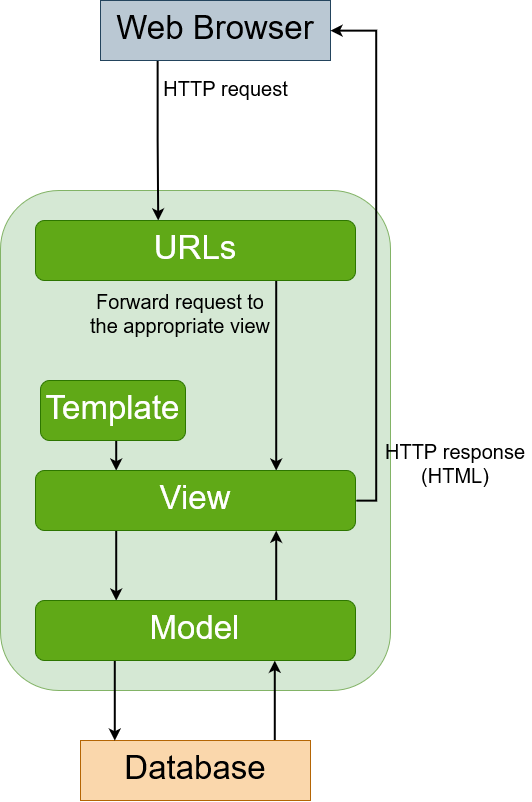
\includegraphics[scale=0.3]{images/Django_doc.png}
    \caption{Schema generico di funzionamento di un applicativo web sviluppato con Django.}
    \label{fig:django_doc}
\end{figure}
\hfill\break
Un'applicazione web in Django tipicamente raggruppa il codice che gestisce questi passaggi in file separati, secondo la 
suddivisione in riquadri verdi della Figura \ref{fig:django_doc} \cite{mdn-django-documentation}, in cui ognuno di questi
gruppi di file svolge delle operazioni ben precise.
\begin{description}
    \item Un \textbf{URL mapper} è usato per reindirizzare le richieste HTTP alla View corretta in base all'URL della richiesta; è possibile processare 
    richieste da qualsiasi URL attraverso una singola funzione, ma è più mantenibile scrivere diverse View per gestire ogni risorsa. 
    Inoltre è possibile controllare se nell'URL è presente un particolare pattern di stringhe o numeri, e passare di conseguenza la richiesta alla 
    funzione appropriata come dati da elaborare.
    \item Una \textbf{View} è una funzione che gestisce le richieste HTTP, e restituisce una risposta HTTP. Le View accedono ai dati necessari per soddisfare la 
    richiesta, anche attraverso i Model, e si delega la formattazione delle risposte ai Template.
    \item I \textbf{Model} sono oggetti in Python che definiscono la struttura dei dati dell'applicazione, e provvedono meccanismi per gestirla (add, modify, 
    delete) e query per interpellare il database.
    \item Un \textbf{Template} è un file di testo che definisce la struttura o il layout di un altro file (come una pagina HTML), attraverso placeholder per
    rappresentare la posizione e il contenuto effettivo. Una View può creare dinamicamente una pagina HTML usando un Template HTML, popolandolo con dati presi dal Model, 
    che a sua volta può recuperli dal database.
\end{description}
Nel Listing \ref{lst:URLex1} si può osservare come viene scritto un URL e come si interfaccia con una View; in questo caso nel 
momento in cui viene fatta una richiesta HTTP a questo URL \textit{recommendation/item/<str:item\_other\_id>/} viene richiamata la 
View \textit{recommendation\_views.item\_recommendation} passando il parametro \textit{<str:item\_other\_id>}.
\lstset{style=python_code_style}
\begin{lstlisting}[language=Python, label=lst:URLex1]
# URL Example 'recommendation/item/35/'
path('recommendation/item/<str:item_other_id>/', recommendation_views.item_recommendation, name='item_recommendation')
\end{lstlisting}
A questo punto, come viene mostrato nel Listing \ref{lst:URLex2}, viene richiamata la View, essa prende i valori che gli vengono passati in ingresso e 
restituisce un risultato, in questo caso viene richiamata la View che implementa il sistema di raccomandazione Item-based, la quale si effettua una ricerca 
nel database per il valore del parametro \textit{<str:item\_other\_id>} in ingresso, verificando l'esistenza di quell'item, questo è possibile
grazie all'ausilio dei Model i quali sono stati utilizzati precedentemente per definire la struttura delle tabelle e dei relativi campi 
contenuti nel database e ora attraverso i cosiddetti QuerySet, messi a disposizione da Django, è possibile accedere a quei dati; successivamente vengono 
determinati tramite l'agoritmo di raccomandazione quali sono i possibili item simili e vengono salvati nella variabile \textit{similar\_item\_evaluations}, 
infine, dopo aver ripulito i dati da informazioni poco rilevanti, viene restiuita una risposta in formato JSON al browser web che ha effettuato la richiesta.
\lstset{style=python_code_style}
\begin{lstlisting}[language=Python, label=lst:URLex2]
# Item recommendation API REST
@api_view(['GET'])
def item_recommendation(request, item_other_id):
    # Trying to retrieve the actual node with item_other_id
    item = Evaluation.objects.get(other_id=item_other_id)

    similar_item_evaluations = item_recommendation_alg(item_other_id)

    # Cleaning the data, deleting all the keys except 'other_id'
    similar_item_evaluations_serilized = EvaluationSerializerRecommendation(similar_item_evaluations, many=True).data

    return JSONResponse(similar_item_evaluations_serilized, safe=False)
\end{lstlisting}
%
\section{Docker}
Docker è una piattaforma software che permette di creare, testare e distribuire applicazioni con la massima rapidità. Docker raccoglie 
le applicazioni in unità standardizzate chiamate \textit{Container} che offrono tutto il necessario per la loro corretta esecuzione, incluse librerie, 
strumenti di sistema, codice e runtime. Con Docker, è possibile distribuire e ricalibrare le risorse per un'applicazione in qualsiasi ambiente, 
tenendo sempre sotto controllo il codice eseguito.\hfill\break
Questa tecnologia utilizza solitamente il kernel di Linux e le sue funzionalità, come Cgroups e namespace, per isolare i processi in modo da poterli 
eseguire in maniera indipendente. Questa indipendenza è l'obbiettivo dei Container: la capacità di eseguire più processi e applicazioni in 
modo separato per sfruttare al meglio l'infrastruttura esistente pur conservando il livello di sicurezza che sarebbe garantito dalla 
presenza di sistemi separati.
%
\begin{figure}[ht!]
    \centering
    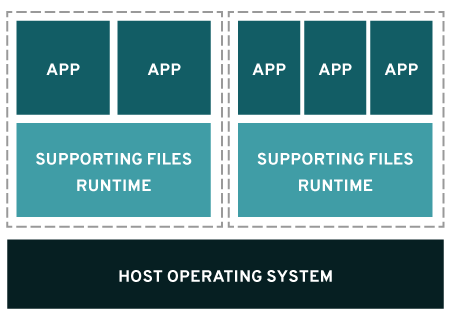
\includegraphics[scale=0.5]{images/Docker_Config_Container.png}
    \caption{Schematizzazione di Container in Docker e di Virtual Machine.}
    \label{fig:DCC}
\end{figure}
\hfill\break
Gli strumenti per la creazione di Container, come Docker, consentono il deployment a partire da un'\textit{immagine}, ciò semplifica la condivisione di 
un'applicazione o di un insieme di servizi, con tutte le loro dipendenze, nei vari ambienti.
Docker, considera i Container come macchine virtuali modulari estremamente leggere, offrendo la flessibilità di creare, distribuire, 
copiare e spostare i Container da un ambiente all'altro, ottimizzando così le app per il cloud.\hfill\break
I Container forniscono una modalità standard per impacchettare il codice delle applicazioni, le configurazioni e le dipendenze, in un singolo oggetto e 
condividono un sistema operativo installato sul server, operando come processi con risorse isolate, assicurando velocità, affidabilità e distribuzioni coerenti, 
indipendentemente dall’ambiente.\hfill\break
%
Questo sistema crea un livello di astrazione fra i Container e il sistema operativo ospitante e gestisce l’attivazione e la disattivazione dei Contenitori. 
Un'altra grande differenza è che la virtualizzazione permette di eseguire più sistemi operativi contemporaneamente in un singolo sistema, mentre i Container 
condividono lo stesso kernel del sistema operativo e isolano i processi applicativi dal resto dell’infrastruttura.
%
\section{Strutture dati gerarchiche}
Nel caso di questa tesi si vogliono memorizzare due tassonomie, aventi struttura ad albero, in cui ogni nodo corrisponde, all'interno di una tabella, ad un 
record; quindi in dati gerarchici si instaurano delle relazioni padre-figlio tra le quali non possono essere rappresentate in modo naturale 
all'interno di un database relazionale, il quale, per l'appunto, segue il Modello Relazionale.\hfill\break
Esso è un modello logico di rappresentazione dei dati all'interno di un database, in cui ogni riga di una tabella è un record identificato univocamente
da una chiave primaria, e le colonne contengono gli attributi dei dati e in genere ogni record ha un valore per ogni attributo.\hfill\break
In questa tesi si è lavorato su un database Sql, in cui i dati normalmente sono conservati come semplici "flat table", e in particolare si è usato il DBMS 
PostgreSQL, un sistema di gestione di database relazionali ad oggetti (ORDBMS). In generale le tabelle contenute in questo tipo di base di dati non permettono la 
memorizzazione secondo un modello gerarchico (come nell'Xml).\hfill\break
Per questo motivo è sorta la necessità di cercare un metodo alternativo per poter rappresentare queste strutture all'interno di database tradizionali.
In questo caso ogni nodo ha un solo padre e nessuno o più figli (a eccezione del nodo radice che non ha un nodo padre); questo genere di rappresentazione 
delle informazioni, può essere trovato in diversi ambiti di applicazione di un database, incluse discussioni su forum e mailing list, 
grafici di organizzazione di un business, categorie per gestire contenuti e prodotti.
%
\begin{figure}[ht!]
    \centering
    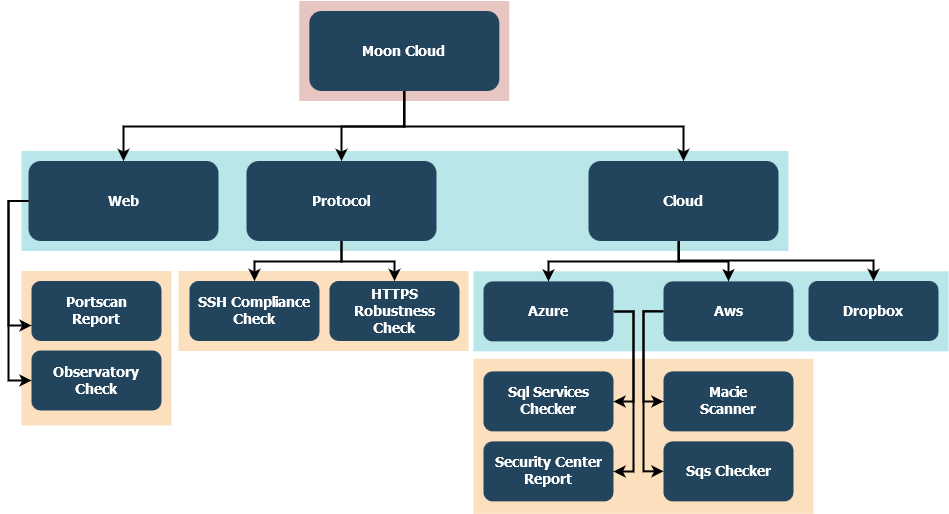
\includegraphics[scale=0.46]{images/MC_Rec_Tree.png}
    \caption{Esempio della rappresentazione gerarchica parziale dei dati nel progetto in questione.}
    \label{fig:MC_Rec_Tree}
\end{figure}
\hfill\break
Durante lo studio compiuto per la realizzazione di questa testi sono stati analizzati diversi approcci per poter gestire le informazioni in modo gerarchico, 
i più importanti presi in considerazione sono i seguenti: 
\begin{itemize}
    \item The Adjacency List Model.
    \item The Nested Set Model.
\end{itemize}
%
\subsection{The Adjacency List Model}
Il primo approccio è chiamato \textit{Adjacency List Model} o metodo ricorsivo; viene definito tale perché il suo funzionamento si basa su una funzione che 
itera per tutto l'albero.\hfill\break
In questo modello, ogni nodo dell'albero contenuto nella tabella ha associato un puntatore al suo nodo padre, e in particolare il nodo radice ha un puntatore 
a un valore NULL per quest'ultimo valore visto che è il nodo di partenza.\hfill\break
La Tabella \ref{table:adjacency_list_model_table} mostra un esempio di possibile rappresentazione parziale dei dati nel database implementato in questo progetto 
secondo questo approccio, utilizzando come riferimento la Figura \ref{fig:MC_Rec_Tree}.
%
\begin{table}[ht!]
\centering
\begin{tabular}[c]{| c | l | c |} 
    \hline
    id & name & parent \\ [0.5ex] 
    \hline
    \rowcolor{rootnodecell} 1 & Moon Cloud & NULL \\ [0.5ex] 
    \rowcolor{categorycell} 2 & Web & 1 \\ [0.5ex] 
    \rowcolor{categorycell} 3 & Protocol & 1 \\ [0.5ex] 
    \rowcolor{categorycell} 4 & Cloud & 1 \\ [0.5ex] 
    \rowcolor{evaluationcell} 5 & Portscan Report & 2 \\ [0.5ex] 
    \rowcolor{evaluationcell} 6 & Observatory Check & 2 \\ [0.5ex] 
    \rowcolor{evaluationcell} 7 & SSH Compliance Check & 3 \\ [0.5ex] 
    \rowcolor{evaluationcell} 8 & HTTPS Robustness Check & 3 \\ [0.5ex] 
    \rowcolor{categorycell} 9 & Azure & 4 \\ [0.5ex] 
    \rowcolor{categorycell} 10 & Aws & 4 \\ [0.5ex] 
    \rowcolor{categorycell} 11 & Dropbox & 4 \\ [0.5ex] 
    \rowcolor{evaluationcell} 12 & Sql Services Checker & 9 \\ [0.5ex] 
    \rowcolor{evaluationcell} 13 & Security Center Report & 9 \\ [0.5ex] 
    \rowcolor{evaluationcell} 14 & Macie Scanner & 10 \\ [0.5ex] 
    \rowcolor{evaluationcell} 15 & Sqs Checker & 10 \\ [0.5ex]
    \hline
\end{tabular}
\caption{Esempio di una possibile tabella per gestire dati in modo gerarchico secondo l'Adjacency List Model.}
\label{table:adjacency_list_model_table}
\end{table}
\hfill\break
Il vantaggio di usare questo modello sta nella sua semplicità di costruzione, soprattutto a livello di codice client-side, 
e di restituzione dei figli di un nodo. Questo approccio diventa problematico nella maggior parte dei linguaggi 
di programmazione perché necessita di una query per ogni nodo dell'albero, e visto che ogni query impiega 
un certo periodo di tempo, questo rende la funzione molto lenta e poco efficiente quando si lavora con alberi di grandi dimensioni. 
Nel Esempio \ref{lst:ex_ALM_query} è possibile osservare come viene recuparata in puro Sql l'intera tassonomia per le Evaluation; 
è possibile notare che la maggiore limitazione di questo approccio è che si necessità di un operazione di JOIN per ogni livello 
della gerarchia, e naturalmente questo porta a un degrado delle performance all'aumentare della complessità; nel caso di questo progetto
si ha una tassonomia a tre livelli, quindi il problema è limitato, ma volendo avere una visione al futuro questo sistema col tempo diventerebbe 
sempre meno performante.
\begin{lstlisting}[language=SQL, label=lst:ex_ALM_query, caption={Query in puro Sql per recuperare l'intera tassonomia delle Evaluation, 
    secondo l'Adjacency List Model.}]
SELECT t1.name AS lev1, t2.name as lev2, t3.name as lev3
    FROM Evaluation AS t1
        LEFT JOIN Evaluation AS t2 ON t2.parent = t1.id
        LEFT JOIN Evaluation AS t3 ON t3.parent = t2.id
    WHERE t1.name = "moon cloud";
\end{lstlisting}
Questa query si può tradurre in codice client-side attraverso una furnzione ricorsiva la quale determina per ogni nodo i suoi figli, per ogni figlio
i suoi figli e così via finchè non si arriva ai nodi foglie.
Inoltre, molti linguaggi non sono ottimizzati per funzioni ricorsive. Per ogni nodo, la funzione crea una nuova istanza di se stessa e 
ogni istanza occupa una porzione di memoria e impiega un certo tempo per inizializzarsi, più grande è l'albero e più questo processo sarà portato a termine 
in maggior tempo.
%
\newpage
%
\subsection{The Nested Set Model}
Il secondo approccio analizzato è il \textit{Nested Set Model}, il quale è stato utilizzato per l'implementazione delle tassonomie per le Evaluation e 
i Controlli (o politiche per verificare il soddisfacimento dei requisiti di sicurezza di un Target o asset indicato dall'utente) all'interno del progetto.\hfill\break
Questo approccio permette di osservare le gerarchie di dati in un modo diverso, non come nodi e linee, come se fosse un albero, ma come container innestati.
%
\begin{figure}[ht!]
    \includegraphics[scale=0.6]{images/MC_Rec_NSM_Container(R).png}
    \caption{Esempio della gestione di dati in modo gerarchico secondo il Nested Set Model, utilizzando quelli presi dal database del 
    progetto in questione (ridotto).}
    \label{fig:MC_Rec_NSM_Container_R}
\end{figure}
\hfill\break
%
Con questo sistema la gerarchia viene mantenuta, secondo il principio cui un nodo padre contiene i suoi figli. Questa struttura 
viene mantenuta in tabella attraverso l'uso di due attributi aggiuntivi, \textit{lft} e \textit{rght}, come è possibile osservare 
dalla Tabella \ref{table:nested_set_model_table} seguente, la quale fa riferimento alla Figura \ref{fig:MC_Rec_NSM_Container} 
posta alla fine della sezione.
%
\newpage
%
\begin{table}[ht!]
\centering
\begin{tabular}[c]{| c | l | c | c |}
    \hline
    id & name & lft & rght \\ [0.5ex] 
    \hline
    \rowcolor{rootnodecell} 1 & Moon Cloud & 1 & 100 \\ [0.5ex] 
    \rowcolor{categorycell} 2 & Web & 86 & 99 \\ [0.5ex] 
    \rowcolor{categorycell} 3 & Protocol & 80 & 85 \\ [0.5ex] 
    \rowcolor{categorycell} 4 & Cloud & 4 & 29 \\ [0.5ex] 
    \rowcolor{evaluationcell} 5 & Portscan Report & 91 & 92 \\ [0.5ex] 
    \rowcolor{evaluationcell} 6 & Observatory Check & 89 & 90 \\ [0.5ex] 
    \rowcolor{evaluationcell} 7 & SSH Compliance Check & 83 & 84 \\ [0.5ex] 
    \rowcolor{evaluationcell} 8 & HTTPS Robustness Check & 81 & 82 \\ [0.5ex] 
    \rowcolor{categorycell} 9 & Azure & 13 & 26 \\ [0.5ex] 
    \rowcolor{categorycell} 10 & Aws & 5 & 12 \\ [0.5ex] 
    \rowcolor{categorycell} 11 & Dropbox & 27 & 28 \\ [0.5ex] 
    \rowcolor{evaluationcell} 12 & Sql Services Checker & 22 & 23 \\ [0.5ex] 
    \rowcolor{evaluationcell} 13 & Security Center Report & 20 & 21 \\ [0.5ex] 
    \rowcolor{evaluationcell} 14 & Macie Scanner & 8 & 9 \\ [0.5ex] 
    \rowcolor{evaluationcell} 15 & Sqs Checker & 10 & 11 \\ [0.5ex]
    \hline
\end{tabular}
\caption{Esempio di una tabella per gestire dati in modo gerarchico secondo il Nested Set Model.}
\label{table:nested_set_model_table}
\end{table}
\hfill\break
Dalla Tabella \ref{table:nested_set_model_table} la gerarchia dei dati viene rappresentata attraverso l'uso 
degli attributi \textit{left} e \textit{right} per rappresentare l'annidamento dei nodi (il nome delle colonne: \textit{left} e \textit{right}, hanno significati 
speciali in Sql; per questo motivo si identificano questi campi con i nomi \textit{lft} e \textit{rght}).
%
\newpage
%
\begin{figure}[ht!]
    \centering
    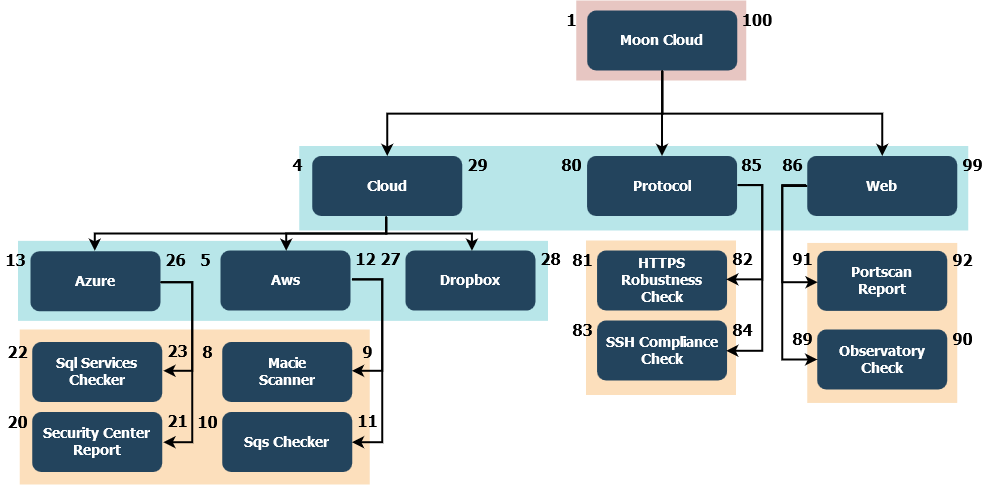
\includegraphics[scale=0.40]{images/MC_Rec_NSM_Tree.png}
    \caption{Esempio della gestione di dati in modo gerarchico secondo il Nested Set Model, utilizzando quelli presi dal database del 
    progetto in questione.}
    \label{fig:MC_Rec_NSM_Tree}
\end{figure}
\hfill\break
L'assegnazione di questi valori viene effettuata ad ogni nodo visitandolo due volte e assegnando i valori in ordine di visita, e in entrambe le visite. 
Quindi vengono associati ad ogni nodo due numeri, memorizzati come due attributi. 
Più precisamente si inizia la visita dell'albero partendo da sinistra e continuando verso destra, un livello alla volta, scendendo per ogni 
nodo i suoi figli, assegnando i valori al campo \textit{left}, prima di assegnare un valore al campo \textit{right}, e successivamente si continua verso 
destra. Questo approccio è chiamato \textit{Modified Preorder Tree Traversal Algorithm} (MPTT). A partire da questa tecnica è stato 
ideata la struttura della tassonomia delle evaluation e dei Controlli implementate nella soluzione proposta in questa tesi, con 
l'ausilio di un package di Python chiamato MPTT, del quale verrà illustrato il funzionamento nel capitolo \ref{chp:04-solution}.\hfill\break
Più semplicemente se si osserva la parte superiore della Figura \ref{fig:MC_Rec_NSM_Container_R} si può notare che la numerazione dei nodi, viene 
effettuata a partire da container più esterno da sinistra e continua verso destra.\hfill\break
A prima vista questo approccio può sembrare più complicato da comprendere rispetto all'Adjacency List Model, ma quest'ultimo è 
molto più veloce quando si vuole recuperare i nodi, visto che basta una query, mentre è più lento per operazioni di inserimento e 
cancellazione dei nodi; il Listing \ref{lst:ex_NSM_query} qui di seguito mostra come è possibile recuperare l'itera tassonomia delle Evaluation; si 
può notare che questa query funziona in modo indipendente dalla profondità della tassonomia; inoltre, non è necessario preoccuparsi del valore \textit{rght} 
del nodo all'interno della clausola \textit{BETWEEN} della query perché il valore cadrà sempre all'interno dello stesso nodo padre come anche il 
valore di \textit{lft}.
\begin{lstlisting}[language=SQL, label=lst:ex_NSM_query, caption={Query in puro Sql per recuperare l'intera tassonomia delle Evaluation, 
    secondo il Nested Set Model.}]
SELECT node.name
    FROM Evaluation AS node, Evaluation AS parent
    WHERE node.lft BETWEEN parent.lft AND parent.rgt
        AND parent.name = "moon cloud"
    ORDER BY node.lft;
\end{lstlisting}
%
Altro esempio è il caso in cui si vuole recuperare tutti i nodi foglia della tassonomia come mostra il Listing \ref{lst:ex_NSM_query2}, in cui è ancora 
più semplice rispetto nell'Adjacency List Model. Nel Nested Set Model, il valori di \textit{lft} e \textit{rght} per i nodi foglia hanno valori 
consecutivi; quindi per trovare i nodi foglia basta cercare quei nodi dove il valore di \textit{rght} è pari a quello di \textit{lft} incrementato di uno.
\begin{lstlisting}[language=SQL, label=lst:ex_NSM_query2, caption={Query in puro Sql per recuperare tutti i nodi foglia della tassonomia delle Evaluation, 
    secondo il Nested Set Model.}]
SELECT name
    FROM Evaluation
    WHERE rgt = lft + 1;
\end{lstlisting}
%
Infine nel caso di inserimento o cancellazione di un nodo il grado di complessità dell'operazione è determinato dalla posizione del nodo che si 
vuole inserire o cancellare; a partire dal caso più semplice, quando si vuole inserire o cancellare un nodo foglia, quel nodo senza figli, fino 
al caso più complesso, quando si vuole cancellare un nodo padre perchè bisogna anche gestire i suoi nodi figli.
Nel primo caso, è sufficente per poter cancellare un nodo senza figli eseguire una query come mostrata nel Listing \ref{lst:ex_NSM_query3}, si determinano 
prima i valori dei campi \textit{lft} e \textit{rght} e la loro differenza, \textit{width}, successivamente cancellato il nodo si sottrae la sua 
differenza da ogni nodo alla sua destra.
\begin{lstlisting}[language=SQL, label=lst:ex_NSM_query3, caption={Query in puro Sql per eliminare un nodo foglia dalla tassonomia delle Evaluation, 
    secondo il Nested Set Model.}]
SELECT @myLeft := lft, @myRight := rgt, @myWidth := rgt - lft + 1
    FROM Evaluation
    WHERE name = "Sqs Checker";

DELETE FROM Evaluation WHERE lft BETWEEN @myLeft AND @myRight;

UPDATE Evaluation SET rgt = rgt - @myWidth WHERE rgt > @myRight;
UPDATE Evaluation SET lft = lft - @myWidth WHERE lft > @myRight;
\end{lstlisting}
%
Nel secondo caso, in cui voglio eliminare il nodo padre ma non i suoi nodi figli si può decidere che i figli vengano spostati allo stesso livello del 
nodo padre eliminato, ciò viene mostrato dal Listing \ref{lst:ex_NSM_query4}. In questo caso si sottrae due da tutti gli elementi a destra di tale nodo 
(visto che i figli avranno una dimensione, \textit{width}, di due) e uno da tutti i nodi che sono suoi figli (per chiudere il gap creato dalla perdita 
del nodo padre e dal valore associato al campo \textit{lft}).
\begin{lstlisting}[language=SQL, label=lst:ex_NSM_query4, caption={Query in puro Sql per eliminare un nodo padre dalla tassonomia delle Evaluation, 
    secondo il Nested Set Model.}]
SELECT @myLeft := lft, @myRight := rgt, @myWidth := rgt - lft + 1
    FROM Evaluation
    WHERE name = "Web";

DELETE FROM Evaluation WHERE lft = @myLeft;

UPDATE Evaluation SET rgt = rgt - 1, lft = lft - 1 WHERE lft BETWEEN @myLeft AND @myRight;
UPDATE Evaluation SET rgt = rgt - 2 WHERE rgt > @myRight;
UPDATE Evaluation SET lft = lft - 2 WHERE lft > @myRight;
\end{lstlisting}
%
\newpage
%
\begin{figure}
    \centering
    \includegraphics[scale=0.49]{images/MC_Rec_NSM_Container.png}
    \caption{Esempio della gestione di dati in modo gerarchico secondo il Nested Set Model, utilizzando quelli presi dal database del 
    progetto in questione.}
    \label{fig:MC_Rec_NSM_Container}
\end{figure}
%
\section{Sistemi di raccomandazione}
Un sistema di raccomandazione (\textit{Recommendation System}) è un sistema che consiglia a un utente uno o più item esistenti 
presenti in un database; l'\textit{item} è inteso come una qualsiasi cosa di interesse all'utente, come prodotti, libri o giornali. 
Quando si esegue una raccomandazione si ha come obbiettivo quello di consigliare l'item che possa essere tra quelli di maggiore 
interesse; in altre parole, devono essere in accordo con i gusti dell'utente.\hfill\break
Oggigiorno si possono trovare due principali trend di sistemi di raccomandazione.
\begin{description}
    \item[Content-based filtering](CBF): un item viene raccomandato ad un utente se esso è simile ad altri item di interesse o piaciuti 
    in passato, prendendo in considerazione prima gli item con alte valutazioni o quelli molto utilizzati; questo è possibile perché ad 
    ogni item sono associate delle informazioni che lo descrivono, e questo insieme di dati viene definito metadati.
    \item[Collaborative filtering](CF): un item viene raccomandato ad un utente se i suoi vicini (altri utenti simili) sono 
    interessati a quello stesso item.
\end{description}
%
\begin{figure}[ht!]
    \centering
    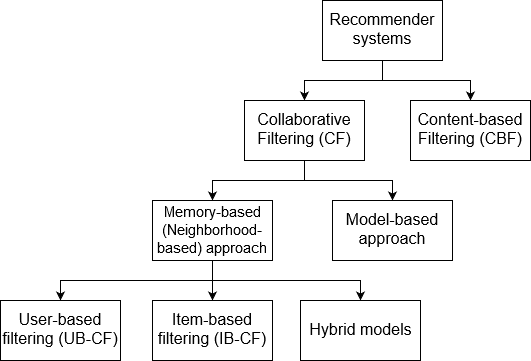
\includegraphics[scale=0.5]{images/recommender_systems.png}
    \caption{Categorizzazione generale dei sistemi di raccomandazione.}
    \label{fig:recommender_systems}
\end{figure}
Entrambi gli approcci hanno i loro punti di forza e di debolezza. Il primo algoritmo si focalizza sul contenuto degli item e 
sugli interessi del singolo utente e propone item differenti a utenti differenti, questo significa che ogni utente può ricevere 
raccomandazioni uniche. 
Tuttavia la più grande limitazione del CBF è il fatto di non poter determinare se un utente è interessato ad un item in modo implicito, 
perché analizza direttamente i metadati del prodotto e non considera gli interessi di altri utenti, i quali potrebbero 
suggerire item che non verrebbero notati con questo approccio.
Per quanto riguarda il CF, nel caso siano presenti molti contenuti e proprietà associati agli item, allora vengono consumate molte 
risorse e tempo per poter analizzarli, nel contempo a questo algoritmo non interessano queste informazioni. Una raccomandazione 
viene fatta sulla base delle valutazioni degli utenti per gli item, o sugli usi che gli utenti fanno degli item e questo è il suo punto 
di forza perché non si trova a dover analizzare item ricchi di informazioni. Allo stesso tempo è anche il suo punto debole, perché può 
portare suggerimenti che potrebbero essere considerati poco adatti sulla base della poca relazione con i profili di alcuni utenti. 
Questo problema è accentuato quando sono presenti nel database molti item che non hanno valutazioni o non sono stati mai usati dagli 
utenti \cite{model-based-approach-for-collaborative-filtering}.
\vspace{0.5 cm}
\hfill\break
Un sistema di raccomandazione filtra i dati usando differenti algoritmi e raccomanda gli item più rilevanti agli utenti attraverso 
un procedimento a 3 fasi.
\begin{description}
    \item[Raccolta di dati:] il primo step è anche quello più importante per poter costruire un sistema di 
    raccomandazione che produca risultanti rilevanti e consistenti. I dati possono essere raccolti in due modi: esplicitamente, 
    cioè attraverso la raccolta diretta di informazioni fornite dagli utenti, ad esempio le valutazioni di un prodotto oppure 
    implicitamente. In questo caso vengono raccolti dati che, non sono prodotti in modo intenzionale dall'utente, ma sono ottenuti 
    dai costanti flussi di dati come la cronologia di ricerca, i click effettuati, lo storico degli ordini, ecc.
    \item[Memorizzazione di dati:] la quantità di dati definisce quanto efficace un modello di raccomandazione possa di 
    diventare. Ad esempio, in un sistema di raccomandazione per film, maggiori sono le valutazioni fornite dagli utenti, e 
    migliore sarà il sistema di raccomandazione per gli altri utenti. Il tipo di dati che si vuole raccogliere determina 
    anche il supporto di memorizzazione più adatto.
    \item[Filtraggio dei dati:] dopo la fase di raccolta e memorizzazione dei dati, essi vanno filtrati per poter estrarre 
    le informazioni rilevanti e poter effettuare le raccomandazioni finali; inoltre, vi sono diversi algoritmi standard per 
    realizzare quest'ultima fase.
\end{description}
%
\subsection{Content-based filtering}
Un Content-based filtering (definito anche con l'acronimo CBF) è un sistema di raccomandazione in cui vengono suggeriti, rispetto ad un item, quelli 
più simili, confrontando le informazioni contenute nei metadati, come una descrizione, uno o più autori, la categoria di 
appartenenza, ecc.. L'idea base che si trova dietro questi sistemi, è il fatto che se ad un utente piace o interessa un particolare 
item allora gli piaceranno anche altri con caratteristiche o proprietà simili.\hfill\break
Questo algoritmo suggerisce prodotti che piacevano all'utente nel passato ed è limitato a item dello stesso tipo. Un 
Content-based recommender fa riferimento a quegli approcci che provvedono raccomandazioni comparano la rappresentazione del 
contenuto che descrive un item e la rappresentazione del contenuto dell'item interessato dall'utente.\hfill\break
Questi metodi sono usati quando si conoscono a priori i metadati sugli item che si vuole suggerire, ma nulla sugli utenti.
In questo sistema, delle \textit{keyword} sono utilizzate per caratterizzare gli item e un profilo dell'utente è 
costruito per memorizzare quali item sono di suo interesse. In altre parole, questi algoritmi cercano di raccomandare quello che 
l'utente ha valutato positivamente o usato nel passato e sta esaminando nel presente. La costruzione del profilo dell'utente, 
spesso temporaneo, non viene basata su un modulo di registrazione che l'utente stesso deve compilare, ma su informazioni 
lasciate indirettamente dall'utente, le quali possono essere: i prodotti che ha maggiormente cercato e acquistato, quelli che sono 
stati inseriti nella lista dei desideri, ecc.. Più precisamente, tra vari item candidati da raccomandare all'utente si passa per un 
processo di confronto con gli item piaciuti dall'utente e gli item migliori vengono suggeriti.
%
\subsection{Collaborative filtering}
Il Filtraggio Collaborativo (definito anche con l'acronimo CF) per poter funzionare, si appoggia ad un database che raccoglie le 
preferenze degli utenti sulla base di un insieme di item, che a loro volta possono essere presenti nella stessa base di dati. 
Si sfruttano tecniche di analisi dei dati per poter ottenere delle raccomandazioni che consiglino gli utenti a trovare gli item 
che gli potrebbero piacere,eventualmente producendo una lista dei migliori N item.\hfill\break
Un utente è sottoposto ad un processo di matching per poter scoprire quali sono i possibili \textit{neighbours}, 
che corrispondono ai possibili utenti aventi storicamente delle preferenze in comune ad egli. Infine, gli item maggiormente 
preferiti dai \textit{neighbours} sono raccomandati all'utente.\hfill\break
Questi sistemi tentano di predire la valutazione o la preferenza che un utente darebbe a un item basandosi sulle preferenze date da altri 
utenti, queste ultime possono essere ottenute o in modo esplicito dagli utenti o tramite misurazioni implicite. 
Inoltre i Filtri Collaborativi non richiedono l'uso di metadati associati agli item, come nei Filtri Content-based.\hfill\break
Tuttavia, restano ancora oggi alcune sfide significative a cui sono sottoposti i sistemi di raccomandazione basati su 
Filtraggio Collaborativo.\hfill\break
Il primo obbiettivo è quello di migliorare la scalabilità di questi algoritmi; essi sono in grado di cercare 
anche diecimila potenziali \textit{neighbours} in tempo reale, ma la richiesta dei sistemi moderni è di cercare dieci milioni 
potenziali \textit{neighbours}, per questo motivo possono nascere problemi di performance con i singoli utenti quando essi hanno 
molte informazioni associate.\hfill\break
Il secondo obbiettivo è quello di migliorare la qualità dei sistemi di raccomandazione per gli utenti. Questi ultimi vogliono 
raccomandazioni di cui possono fidarsi e che possono aiutarli a trovare item di loro gusto e interesse. 
Per certi versi questi due obbiettivi sono in conflitto tra di loro; per ottenere dei risultati validi e di una certa importanza è 
necessario trattarli in contemporanea perché aumentare solamente la scalabilità diminuirebbe la qualità delle raccomandazioni e viceversa 
\cite{item-based-collaborative-filtering}.\hfill\break
Il principale modello di Filtri Collaborativi studiato in questo elaborato e approfondito nel capitolo successivo, è il metodo definito 
come \textit{Memory-based} e il vantaggio di utilizzare questa tecnica sta nel fatto di essere semplici da implementare e i risultati 
ottenuti sono altrettanto semplici da interpretare; mentre si possono trovare anche Filtri Collaborativi che sfruttano metodi 
\textit{Model-based} che si basano sulla fattorizzazione di matrici e sono molto più funzionali per gestire il problema della 
sparsità dei dati. Questi ultimi sono sviluppati usando algoritmi di data mining e machine learning per predire le valutazioni di utenti 
su item senza valutazioni, tentando di comprimere grandi database in un modello ed effettuare il processo di raccomandazione applicando dei 
meccanismi di riferimento all'interno di questo modello, questo permette ai CF Model-based di rispondere alle richieste degli utenti 
istantaneamente \cite{model-based-approach-for-collaborative-filtering}.
%
\subsection{Il problema della Cold Start}
Cosa succederebbe se un nuovo utente o un nuovo item venisse aggiunto al database? Questa situazione è chiamata \textit{Cold Start} ed 
è possibile trovarne di due tipi.
\begin{description}
    \item[Visitor Cold Start:] si verifica quando un nuovo utente viene aggiunto al database, e visto che non è presente alcuno storico relativo, 
    il sistema non è a conoscenza delle sue preferenze; per questo motivo diventa molto più difficile raccomandare prodotti a quel particolare utente. 
    Per risolvere questo problema, a livello teorico, si potrebbe applicare un procedimento di raccomandazione basata sulla popolarità dei prodotti, ma 
    solo una volta che si è venuti a conoscenza delle preferenze dell'utente, sarà possibile generare delle raccomandazioni più precise e adeguate 
    alle sue esigenze.
    \item[Item Cold Start:] si verifica quando un nuovo item viene inserito nel sistema. L'azione dell'utente è quella più importante per determinare 
    il valore di questo item all'interno dell'ecosistema; quindi maggiore è l'interazione che un item riceve maggiore è la facilità che venga raccomandato 
    all'utente interessato.
\end{description}
